%\chapter{The Optimum Receiver}

\subsection{The Gaussian Distribution}
\begin{problem}
\label{ch1_prob1}
Generate a Gaussian random number with 0 mean and unit variance.
\end{problem}
%
\solution Open a text editor and type the following program.

%%
\lstinputlisting{./chapter1/codes/1.1.py}
%%
Save the file as gaussian\_no.py and run the program.
%
\begin{problem}
The mean of a random variable $X$ is defined as
%
\begin{equation}
E\sbrak{X} = \frac{1}{N}\sum_{i=1}^{N}X_i
\end{equation}
%
and its variance as
%
\begin{equation}
\text{var}\sbrak{X} = E\sbrak{X- E\sbrak{X}}^2 
\end{equation}
%
Verify that the program in \ref{ch1_prob1} actually generates a Gaussian random variable with 0 mean and unit variance.
\end{problem}
\solution  Use the header in the previous program, type the following code and execute.
\lstinputlisting{./chapter1/codes/1.2.py}
%
%
\begin{problem}
Using the previous program, verify you results for different values of the mean and variance.
\end{problem}

\subsection{CDF and PDF}
\begin{problem}
A Gaussian random variable $X$ with mean 0 and unit variance can be expressed as $X \sim \mathcal{N}\brak{0,1}$. Its cumulative distribution function (CDF) is defined as
\begin{equation}
F_X(x) = \pr{X < x}, 
\end{equation}
Plot $F_X(x)$.
\end{problem}
\solution  The following code yields Fig. \ref{ch1_prob3_fig}.
\lstinputlisting{./chapter1/codes/1.3.py}
%
\begin{figure}
\centering
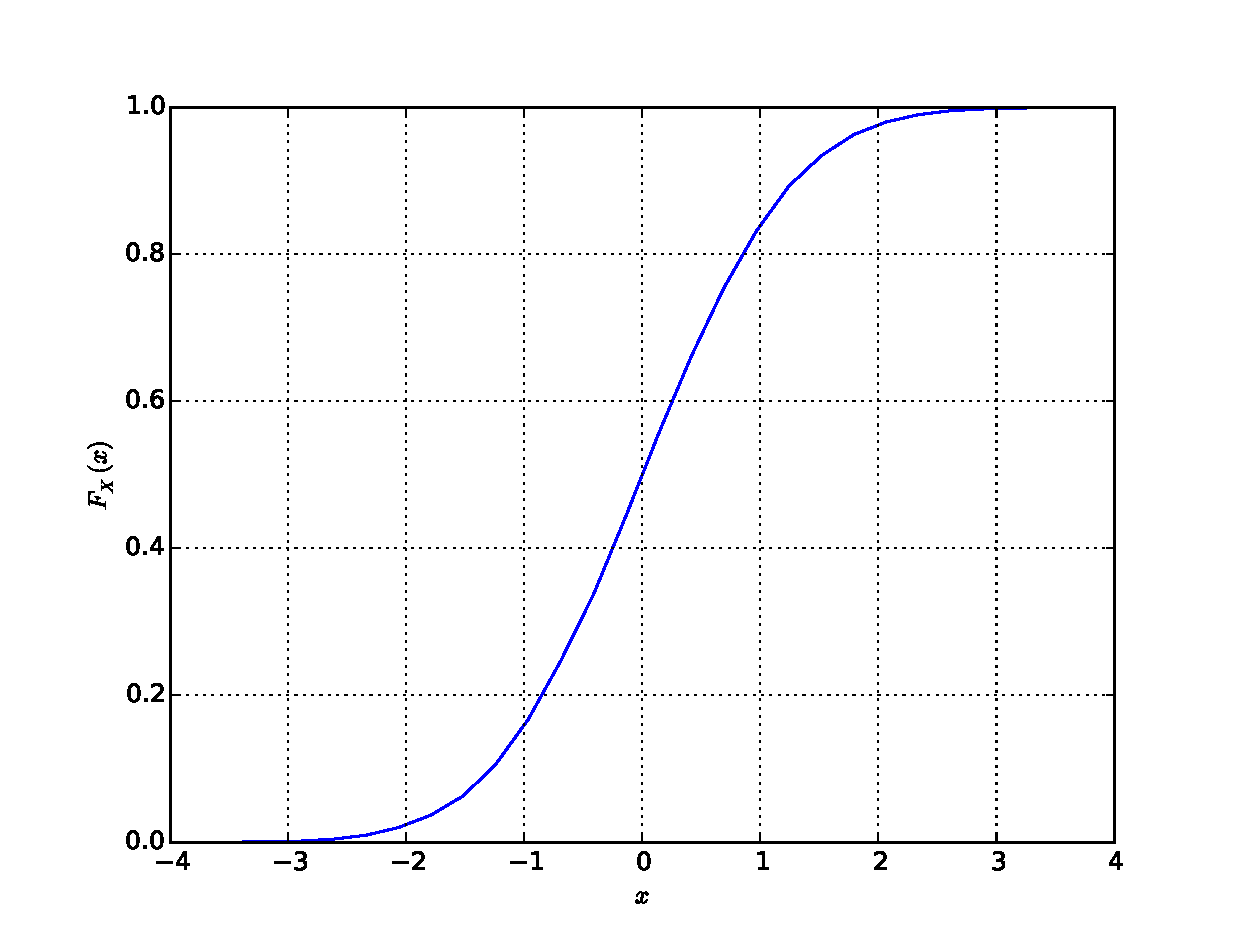
\includegraphics[width=\columnwidth]{./chapter1/figs/ch1_prob3_fig}
\caption{CDF of $X$}
\label{ch1_prob3_fig}
\end{figure}
%
\begin{problem}
List the properties of $F_X(x)$ based on Fig. \ref{ch1_prob3_fig}.
\end{problem}
%
\begin{problem}
Let
%
\begin{equation}
p_{X}(x_i) = \frac{F_{X}(x_i)-F_{X}(x_{i-1})}{h}, i = 1, 2, \dots
{h}
\end{equation}
%
for $x_i = x_{i-1}+h, x_1 = -4$. Plot $p_X(x_i)$.  On the same graph, plot
%
\begin{equation}
p_{X}(x) = \frac{1}{\sqrt{2\pi}}e^{-x^2/2}, - 4 < x < 4
\end{equation}
%
\end{problem}
%
\solution The following code yields the graph in Fig. \ref{ch1_prob4_fig}
\lstinputlisting{./chapter1/codes/1.4.py}
\begin{figure}
\centering
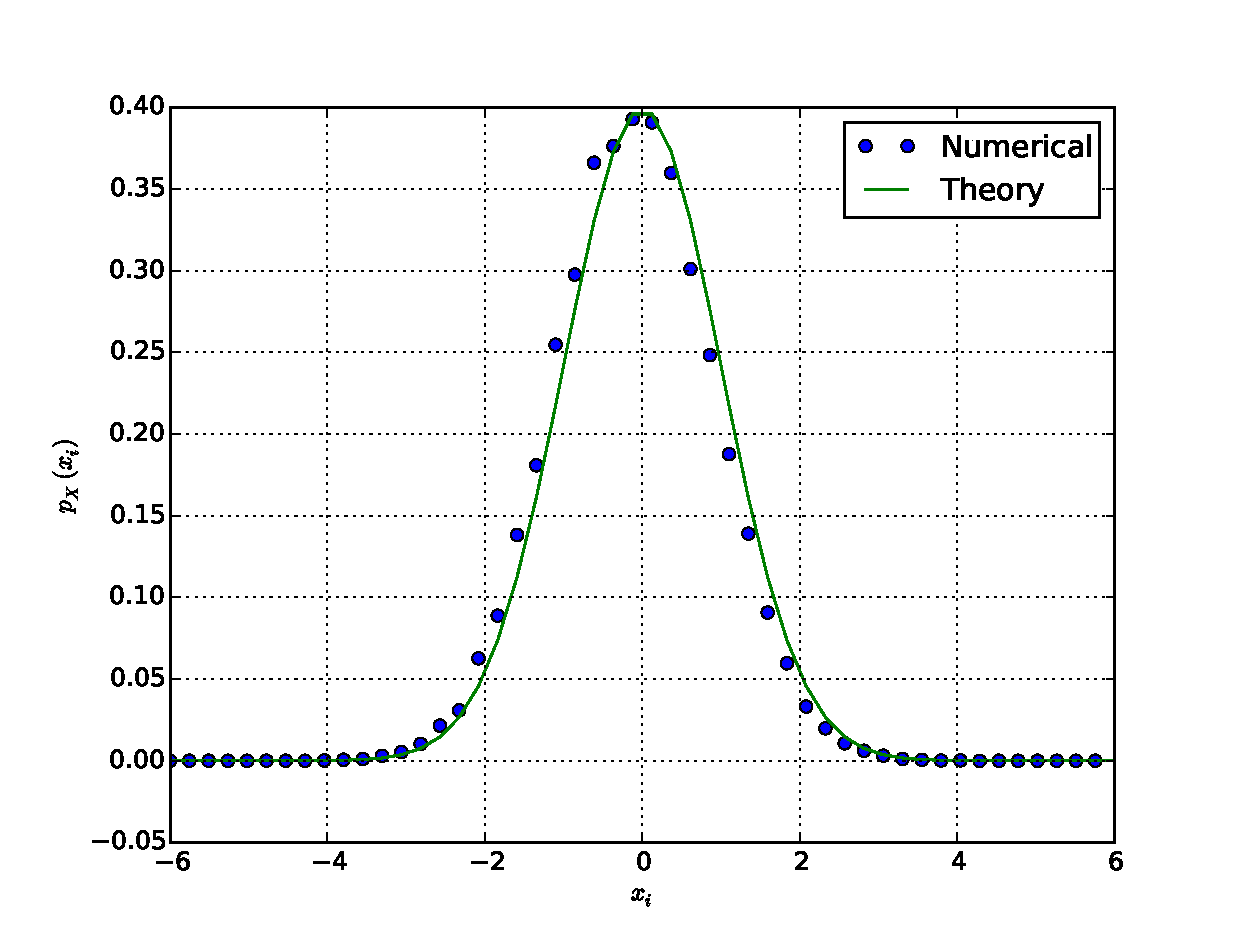
\includegraphics[width=\columnwidth]{./chapter1/figs/ch1_prob4_fig}
\caption{The PDF of $X$}
\label{ch1_prob4_fig}
\end{figure}
%
Thus, the PDF is the derivative of the CDF.  For $X\sim \mathcal{N}\brak{0,1}$, the PDF is
%
\begin{equation}
p_{X}(x) = \frac{1}{\sqrt{2\pi}}e^{-\frac{x^2}{2}}, \quad -\infty < x < \infty
\end{equation}
\begin{problem}
%
For $X\sim \mathcal{N}\brak{\mu,\sigma^2}$,
\begin{equation}
p_{X}(x) = \frac{1}{\sqrt{2\pi}\sigma}e^{-\frac{\brak{x-\mu}^2}{2\sigma^2}}, \quad -\infty < x < \infty
\end{equation}
Plot $p_{X}(x)$ for different values of $\mu$ and $\sigma$ in the same graph.  Comment.
\end{problem}







 




 




